\documentclass[UTF8,a4paper]{ctexart}
\usepackage[margin=1in]{geometry}
\usepackage{fancyhdr,hyperref,float,graphicx,color,amsmath}
\pagestyle{fancy}
\hypersetup{hidelinks}

\lhead{\bfseries \leftmark}
\chead{}
\rhead{SCUT}
\lfoot{\url{https://github.com/285571052}}
\cfoot{qhy}
\rfoot{\thepage}
\setlength{\headheight}{13pt}
\renewcommand{\headrulewidth}{0.4pt}
\renewcommand{\footrulewidth}{0.4pt}

\setlength{\parindent}{0pt}
\newcommand{\spaceline}{\vspace{\baselineskip}}

\author{ qhy }
\date{\today}
\title{操作系统}

\begin{document}
  \maketitle
  \tableofcontents
  \newpage

  \section{介绍}

  操作系统为童虎提供良好的用户接口

  操作系统是一个资源管理器,对多进程以及资源(共享)进行控制

  \section{进程与线程}
  {\color{blue}分三次课讲}

  \textbf{进程的创建时间:}
  \begin{itemize}
    \item 系统启动,reboot
    \item 命令行或打开图标
    \item fork(),创建子进程
    \item 启动一个批处理(batch job)
  \end{itemize}

  {\color{blue}命令行后面加个$\&$ 表示后台运行}

  \spaceline
  \textbf{进程的终止:}
  \begin{itemize}
    \item 正常退出,Normal exit\\
    end of main
    \item 错误终止 error exit\\
    exit(2)
    \item 致命错误,Fatal error\\
    除0等
    \item 被终止,kill by another process\\
    kill pid
  \end{itemize}

  \textbf{用户与程序的关系:}
  用户启动程序,有两种情况:
  \begin{itemize}
    \item 多个用户启动多个程序
    \item 多个用户共享一个实例
  \end{itemize}

  \textbf{实例:}一个实例对应一个进程 , 一个进程可以对应多个程序。

  {\color{blue}查看进程:
  \begin{itemize}
    \item Linux\\
    ps -e
    \item Windows\\
    ctrl + alt + delete
  \end{itemize}}

  \subsection{进程模型}
  主要有两种分类:
  \begin{itemize}
    \item 多进程,串行运行
    \item 多进程,并行运行\\
    实际上是多个进程交替运行一段时间,在单处理器机器上,本质上还是串行运行
    ,即某个时间点只有一个程序运行(分时运行)
  \end{itemize}

  \textbf{进程的层次结构:}父进程可以创建子进程,子进程也可以创建它的子进程。

  若一堆进程有同一个父进程,则称为进程组。

  进程的状态:
  \begin{figure}[H]
    \centering
    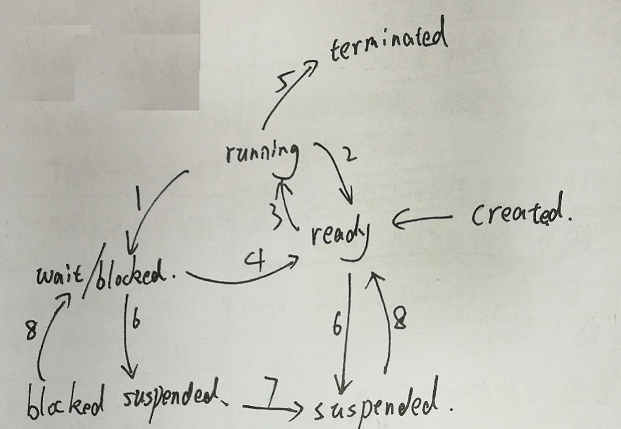
\includegraphics[scale = 0.3]{assets/caozuoxitong_fe21f.png}
    \caption{进程的状态}
  \end{figure}

  \begin{itemize}
    \item [0.] 创建进程
    \item [1.] 阻塞状态\\
    等待非CPU资源的申请,如I/O的申请
    \item [2.] 停止运行当前进程,运行其他进程
    \item [3.] 运行当前程序
    \item [4.] 一切准备就绪(申请得到资源等),等待运行(等待CPU时间分配)
    \item [5.] 进程终止
    \item [6.] 进程挂起\\
    (当内存紧张时)先把进程非运行着的进程放一边去
    \item [7.] 等待的设备已经可用,不会直接进入ready而是进入suspended
    \item [8.] 唤醒

  \end{itemize}

    \subsection{地址空间}
    一般情况,内核空间的地址较大,而用户空间的地址较小。比如
    \begin{tabular}{|c|}
      \hline\\
      $0xFFFF\cdots$内核空间\\
      $stack$\\
      $\cdots$\\
      $heap$\\
      $0x0000\cdots$用户空间(code和data)\\
      \hline
    \end{tabular}
    即,用户代码与数据 和 内核代码 分别放在地址空间两端,而堆和栈则放在次两端, 这样就能保证堆和栈在增长的时候
    有空间可以用,而无需拷贝移动到更大的地址空间中。

    \spaceline
    \textbf{程序区段:}
    \begin{itemize}
      \item Text
      \item Data
      \item Stack
      \item Heap
    \end{itemize}

    \subsection{进程控制块(Process Control Block ,PCB)}

    \textbf{PCB:}记录进程相关的信息,见图\ref{fig-PCB}

    \begin{figure}[H]
      \centering
      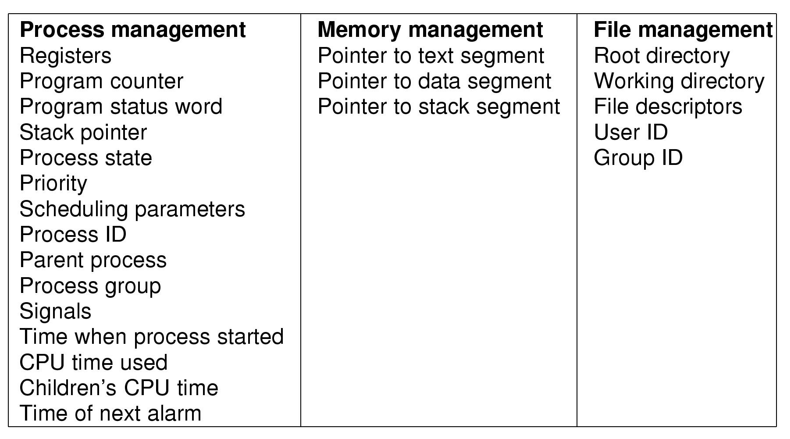
\includegraphics[scale = 0.45]{assets/ModernOperatingSystems_fe620.png}
      \caption{Process Control Block}
      \label{fig-PCB}
    \end{figure}
    {\color{red} 貌似没有保存堆相关的信息?然后栈虽然保存了,但是在实际进程切换的过程中,它是怎么处理的呢?}

    \subsection{上下文切换 Context Switch}
    \textbf{上下文切换}:切换CPU的进程,主要分为以下几个步骤。
    \begin{itemize}
      \item 保存旧进程的PCB
      \item 载入新进程的PCB
      \item 刷新缓存Cache
      \item 改变内存映射表(TLB)
    \end{itemize}

    \textbf{CPU利用率:}直接定义是$\frac{\text{CPU有效时间}}{\text{CPU总时间}}$,$1 - p^n$,其中$p$为一个进程等待$I/O$的时间与其停留在内存时间的比,n为同在内存的进程数。
    {\color{blue}这个n次方怎么理解?p表示一个进程没有利用到CPU的时间的比例, 但是这个比例中,有部分是被其他进程所使用的
    ,因此再乘上其他进程没用到的比例才是CPU总体没被利用的比例,这里去了近似,所有的进程未利用的比例都是p,因此是$p^n$}

    \subsection{线程 Thread}
    \textbf{线程:}
    \begin{itemize}
      \item 轻量级进程 Lightweight Process
      \item 一个进程可以同时做多件事情
      \item 同进程的线程可以共享进程内的相同资源
      \item 每个线程都有自己的栈空间\\
      因为并行处理,栈空间是不能共享的,否则会发生冲突。\\
      {\color{blue}那么问题来了,栈到底是怎么实现的?其实就是取一块内存块作为栈空间,因此栈的大小并不是无限大的,而是有限制的
      ,这也是为什么会存在爆栈的现象。
      }
    \end{itemize}

    \textbf{POSIX线程标准:}某个线程标准,在C中使用\textbf{pthread.h}调用相关函数。

    \spaceline
    \textbf{线程的实现方式:}
    \begin{itemize}
      \item 在用户空间中实现线程(Old linux)\\
      即线程表放在用户空间中,调用一个进程,运行的是线程。\\
      内核对线程一无所知。
      \item 在内核空间中实现(Windows XP/2000)\\
      即线程表放在内核中,由内核来管理线程。
      \item 上面两种的混合型(Solaris)\\
      用户级线程与内核线程多路复用。\\
      一个内核线程可以对应多个用户线程。{\color{red}什么意思?}
    \end{itemize}

    \textbf{调度程序激活机制:}尽管内核级线程在一个关键点上优于用户级线程,但是内核线程速度慢,因此采用调度程序激活机制来
    保持优良特性的情况下改进速度。

    {\color{red}内核级线程有什么优良特性?后面再补充这一方面的内容。}

    \spaceline
    \textbf{弹出式线程}
    {\color{red}后面再补充这一方面的内容。}

    \spaceline
    \textbf{作业:P95-97 , 1 , 6 ,7 11,12}

    \spaceline
    \textbf{等待时间:}到任务启动的时间\\
    \textbf{周转时间:}等待时间+任务执行时间

    \spaceline
    \textbf{老化算法:}预测下一次任务的执行时间,计算方法是前两次的时间之和乘以老化因子,然后结果再和下一个时间重复操作。

    \subsection{调度}
    \textbf{为什么需要调度?}\\
    当计算机系统是多道程序设计系统时,通常就会有多个进程或县城同时竞争 CPU ,只要有两个或更多的进程处于就绪
    状态,这种情形就会发生。如果只有一个CPU可用,那么久必须选择下一个要运行的进程。在操作系统中,完成选择工作
    的一部分就称为\textbf{调度程序(scheduler)},该程序使用的算法称为\textbf{调度算法(scheduling algorithm)}

    \spaceline
    \textbf{抢占式调度与非抢占式调度:}
    \begin{itemize}
      \item 抢占式调度(非当前运行着的进程控制)\\
      抢占主要体现在CPU选择下一个任务的时候,某些任务优先占有的CPU。\\
      分为两个阶段,首先是运行程序被强行中断至就绪状态(或者运行程序运行完毕或阻塞),\\
      然后优先级\footnote{优先级:这里的优先级是广义上的优先级,不一定是指一个数字什么的,也可以是其他的量}高的进程。

      \item 非抢占式调度\\
      同优先级的任务,按照某种规则进行调度。\\
      主要有两个方面,一个是是资源放弃,一个是按规则使用。\\
      程序运行到终止或阻塞时,自愿放弃对CPU的占用\\
      或者当前运行的程序CPU时间用完,被强制中断后,同优先级的处于队列首的进程接着占用CPU
    \end{itemize}

    \spaceline
    \textbf{进程的行为:}
    \begin{itemize}
      \item 长时间占有CPU-计算密集型
      \item 短时间占有CPU-I/O密集型
    \end{itemize}

    \spaceline
    \textbf{何时调度?执行调度程序的时机?}
    \begin{itemize}
      \item 进程创建/终止
      \item O/O中断
      \item 运行中的进程被阻塞
      \item 时钟中断
    \end{itemize}

    \spaceline
    \textbf{调度需要考虑的因素:}
    \begin{itemize}
      \item 公平
      \item CPU利用率
      \item 周转时间\\
      等待和执行完成所花费的时间。
      \item 等待时间\\
      从进入任务列表到开始执行的等待时间
      \item 响应时间{\color{red} ????后面进行补充}
      \item 调度的策略
      \item 截止时间\\要求在截止时间内完成作业
    \end{itemize}

    \spaceline
    按照运行的环境,\textbf{主要可以划分成3类:}
    \begin{itemize}
      \item 批处理系统\\
      要求最大吞吐量,最小周转时间,同时CPU利用率高\\
      批处理系统中,每个任务都是严格按顺序执行,每个任务都是\textbf{一次性完成}\\
      即轮到任务1,只有任务1完成了之后才进行下一个任务。(基本单元是一个完整的任务)
      \item 交互式系统\\
      要求最小响应时间\\
      在实现上,把CPU划分成若干个时间片,再按一定规则对时间片进行分配。\\
      注意,按时间片执行,也就意味着,一个时间片内不一定能完成一个任务。(基本单元是一个CPU时间片)
      \item 实时系统\\
      在截止时间之前要完成作业
    \end{itemize}

    \spaceline
    \textbf{批处理系统中的调度:}
    \begin{itemize}
      \item 先来先服务\\
      先到的任务先处理,使用队列实现
      \item 最短作业优先\\
      \item 最短剩余时间优先\\
      在没有新任务的时候,这个和上一个调度室完全一样的。\\
      当新任务进入时,如果新任务的剩余时间比当前运行着的任务还要少,那么立刻挂起当前任务,
      转去执行新来的,剩余时间更少的任务
    \end{itemize}

    \spaceline
    \textbf{交互式系统}
    \begin{itemize}
      \item 转轮调度\\
      每个任务按队列顺序一次使用时间片,使用完之后进入队尾直到任务完成。\\
      时间片设得太短会导致过多的进程切换,降低了CPU的效率;而设得太长又可能引起对短的交互请求的响应时间变长。\\
      将时间片设为20ms$~$50ms通常是一个比较合理得折中。

      \item 优先级调度
      高优先级的先占用CPU\\
      为了防止高优先级进程无休止地运行下去,调度程序可以在每个时钟滴答(即每个时钟中断)降低当前进程的优先级。\\
      UNIX优先级:$pri = 40 + nice + \frac{cpu}{2}$

      \item 多级队列
      与优先级的思想类似,但是这里的优先级不是体现在优先占用CPU时间,而是不同优先级,连续占用CPU时间片的数目不一样。\\
      比如,最高级优先级的进程运行一个时间片,次高的运行2个时间片,以此类推\\
      那么如果确定优先级?\\
      一个进程初次被分配一个时间片,再次被分配两个,接着更多。\\
      (这也是为什么次高的进程反而占有的时间片更长了,因此,占用CPU的次数越多,说明这个进程需要的时间越长)\\
      除此之外,也可以通过其他姿势调整优先级。

      \item 最短进程优先\\
      选择最短作业的进程运行。\\
      问题是,如何从当前可运行的进程中找出最短的那一个进程?\\
      一种办法是根绝进程过去的行为进行预测。\\
      \textbf{老化算法:}假设某个终端上每条命令的运行时间为$T_0$,现在假设测量其下次运行时间为$T_1$
      ,可以用着两个值得加权和来改进估计时间,即$aT_0 + (1 - a)T_1$

      \item 保证调度\\
      保证调度考虑的因素和前面不同,这个调度是向进程作出明确的性能保证。即如果进程是等价的,那么要保证这些进程占有的CPU时间相同\\
      由于各个进程实际获得的CPU时间是已知的,所以很容易计算出真正获得的CPU时间和应获得的CPU时间(对进程的保证)之比。\\
      比率为0.5说明一个进程只获得应得时间的一半,而比率为2.0则说明它获得应得时间的2倍。\\
      于是该算法随后转向比率最低的进程,直到该进程的比率超过它的最接近竞争者为止。

      \item 彩票调度\\
      每个进程都分配到彩票,中彩票的进程获得CPU时间。\\
      可以通过控制进程获得的彩票的数目来控制占用CPU时间的比例。\\
      还有其他玩法,对于协同进程可以集合彩票一起用\\
      比如A必须等待B进程完成才能继续,A可以把票给B使得B能更多占有CPU时间

      \item 公平分享调度\\
      和保证调度的思想有点类似,不过公平分享调度是针对用户而非进程。\\
      前面的调度都是针对进程而言的,如果用户1启动9个进程,而用户2启动了一个进程。\\
      这样用户1得到90\%的CPU时间,而用户2得到了10\%的CPU时间,显然是不公平的。\\
      为了避免这种情况,某些系统在调度处理之前考虑谁拥有进程这一因素,在这种模式中,
      每个用户分配到CPU时间的一部分,而调度程序以一种强制的方式选择进程。\\
      比如前2个CPU时间片给用户1的进程,后2个CPU时间片给用户2的进程。\\
      当然也可以使用类似保证调度的思想,这取决于对\textbf{公平}的含义。

    \end{itemize}

    注:可以使用\textbf{平均等待时间}来衡量每个调度的优劣

    \spaceline
    \textbf{多CPU的调度:}
    \begin{itemize}
      \item 自调用\\
      每个CPU有自己的调度队列,任务分配到哪个CPU就在哪个CPU上运行。
      \item 主从式调度\\
      一个CPU运行调度程序控制其他CPU的调度,其他CPU运行被分配的任务。
      \item 非对称式\\
      某些CPU专门做某个单一的工作。\\
      比叡一个CPU专门处理网络,其他CPU处理其他任务。
      \item Gang调度\\
      对进程进行分组,以组为单位进行调度。\\
      组内的一个进程被挂起,组内的其他进程也终止。\\
      比如,send和receive两个进程,如果send被挂起不再发送,那么receive进程也没必要继续运行。
    \end{itemize}

    \spaceline
    \textbf{优先级倒置:}在调度的时候可能会出现优先级倒置的现象,比如优先级高的进程需要访问或修改内核的某些数据,\\
    而这些数据又恰巧被优先级低的进程占用而无法使用,那么优先级高的进程就需要等待优先级低的进程完成之后才能继续任务。
    这就导致优先级高的进程受制于优先级低的进程,优先级实际上并不起作用。

    \textbf{解决办法:优先级继承}:优先级低的进程继承高优先级进程的优先级,直到高优先级进程完成任务。

    \spaceline
    \textbf{实时系统:}\\
    实时系统通常可以分为\textbf{硬实时}和\textbf{软实时},前者的含义是必须满足绝对的截止时间,
    后者的含义是虽然不希望偶尔错失截止时间,但是可以容忍。

    \spaceline
    实时系统中的事件可以按照响应方式进一步分类为\textbf{周期性}(以规则的时间间隔发生)事件或\textbf{非周期}
    (发生时间不可预知)时间。\\
    如果有$m$个周期事件,事件$i$以周期$P_i$发生,并需要$C_i$秒CPU时间处理一个事件,那么可以处理负载的条件是
    \[\sum_{i = 1}^m \frac{C_i}{P_i} \leq 1\]
    满足这个条件的实时系统,称为\textbf{是可调度的}。

    \spaceline
    \textbf{策略与机制}:调度机制位于内核,而调度策略由用户进程决定。

    \subsection{进程间通信,Inter Process Communication , IPC}

    进程间通讯主要有3个问题:
    \begin{itemize}
      \item 进程如何把信息传递给另一个进程
      \item 确保两个或更多的进程在关键活动中不会出现交叉。
      \item 与正确的顺序有关(如果该顺序是有关联的话)
    \end{itemize}

    进程间通讯的解决方案,同样适用于线程间通讯。

    {\color{blue}Murphy 法则:任何可能出错的地方终将出错。}

    \subsubsection{数据竞争}
    多进程进程数据共享的时候,可能会出现数据竞争的问题。

    其中一个解决办法是,建立临界区\footnote{\textbf{临界区:对共享内存进行访问的程序片段。}}
    ,对进程适当地安排,使得两个进程不可能同时处于临界区内。(即同一时间,只有一块代码(临界区)能操作临界资源)

    对于一个好的解决方案,临界区需要满足一下4个条件:
    \begin{itemize}
      \item 任何两个进程不能同时处于其临界区(互斥)
      \item 不应对CPU的速度和数量做任何假设
      \item 临界区外运行的进程不得阻塞其他进程菊(有闲让进)
      \item 不得使进程无限期等待进入临界区(有限等待)
    \end{itemize}

    \subsubsection{忙等待的互斥}
    \textbf{忙}体现在,当一个进程想要进入临界区,先检查是否允许进入,若不允许,则该程序将原地等待,直到允许为止。

    这种方法不仅浪费了CPU时间,而且可能引起优先级倒置等问题,但是如果切换上下文的时间开销大于忙等待的话,还是选择忙等待好。

    忙等主要有以下6类:
    \begin{itemize}
      \item 屏蔽中断\\
      使每个进程在刚刚进入临界区后立即屏蔽所有中断,并在就要离开之前再打开中断。\\
      屏蔽中断使系统底层的调用,不适合用户操控,而适合操作系统控制。\\
      并且,对于多CPU的情况下,disable指令只对执行这个指令的CPU有效。
      \item 锁变量\\
      就是不断循环判断,直到满足变量为某个值的条件。\\
      这个方法判断的读取,和进入循环后的修改是分两步进行的,可能会被其他进程中断,进而导致冲突。
      \item 严格轮换法\\
      每个进程轮流访问,当时不适合一个进程比另一个进程慢很多的情况。\\
      尽管该算法避免了所有的竞争可能,但是它违背了临界区的条件3,所以不是一个好的方案
      \item Peterson解法
      \begin{figure}[H]\centering
        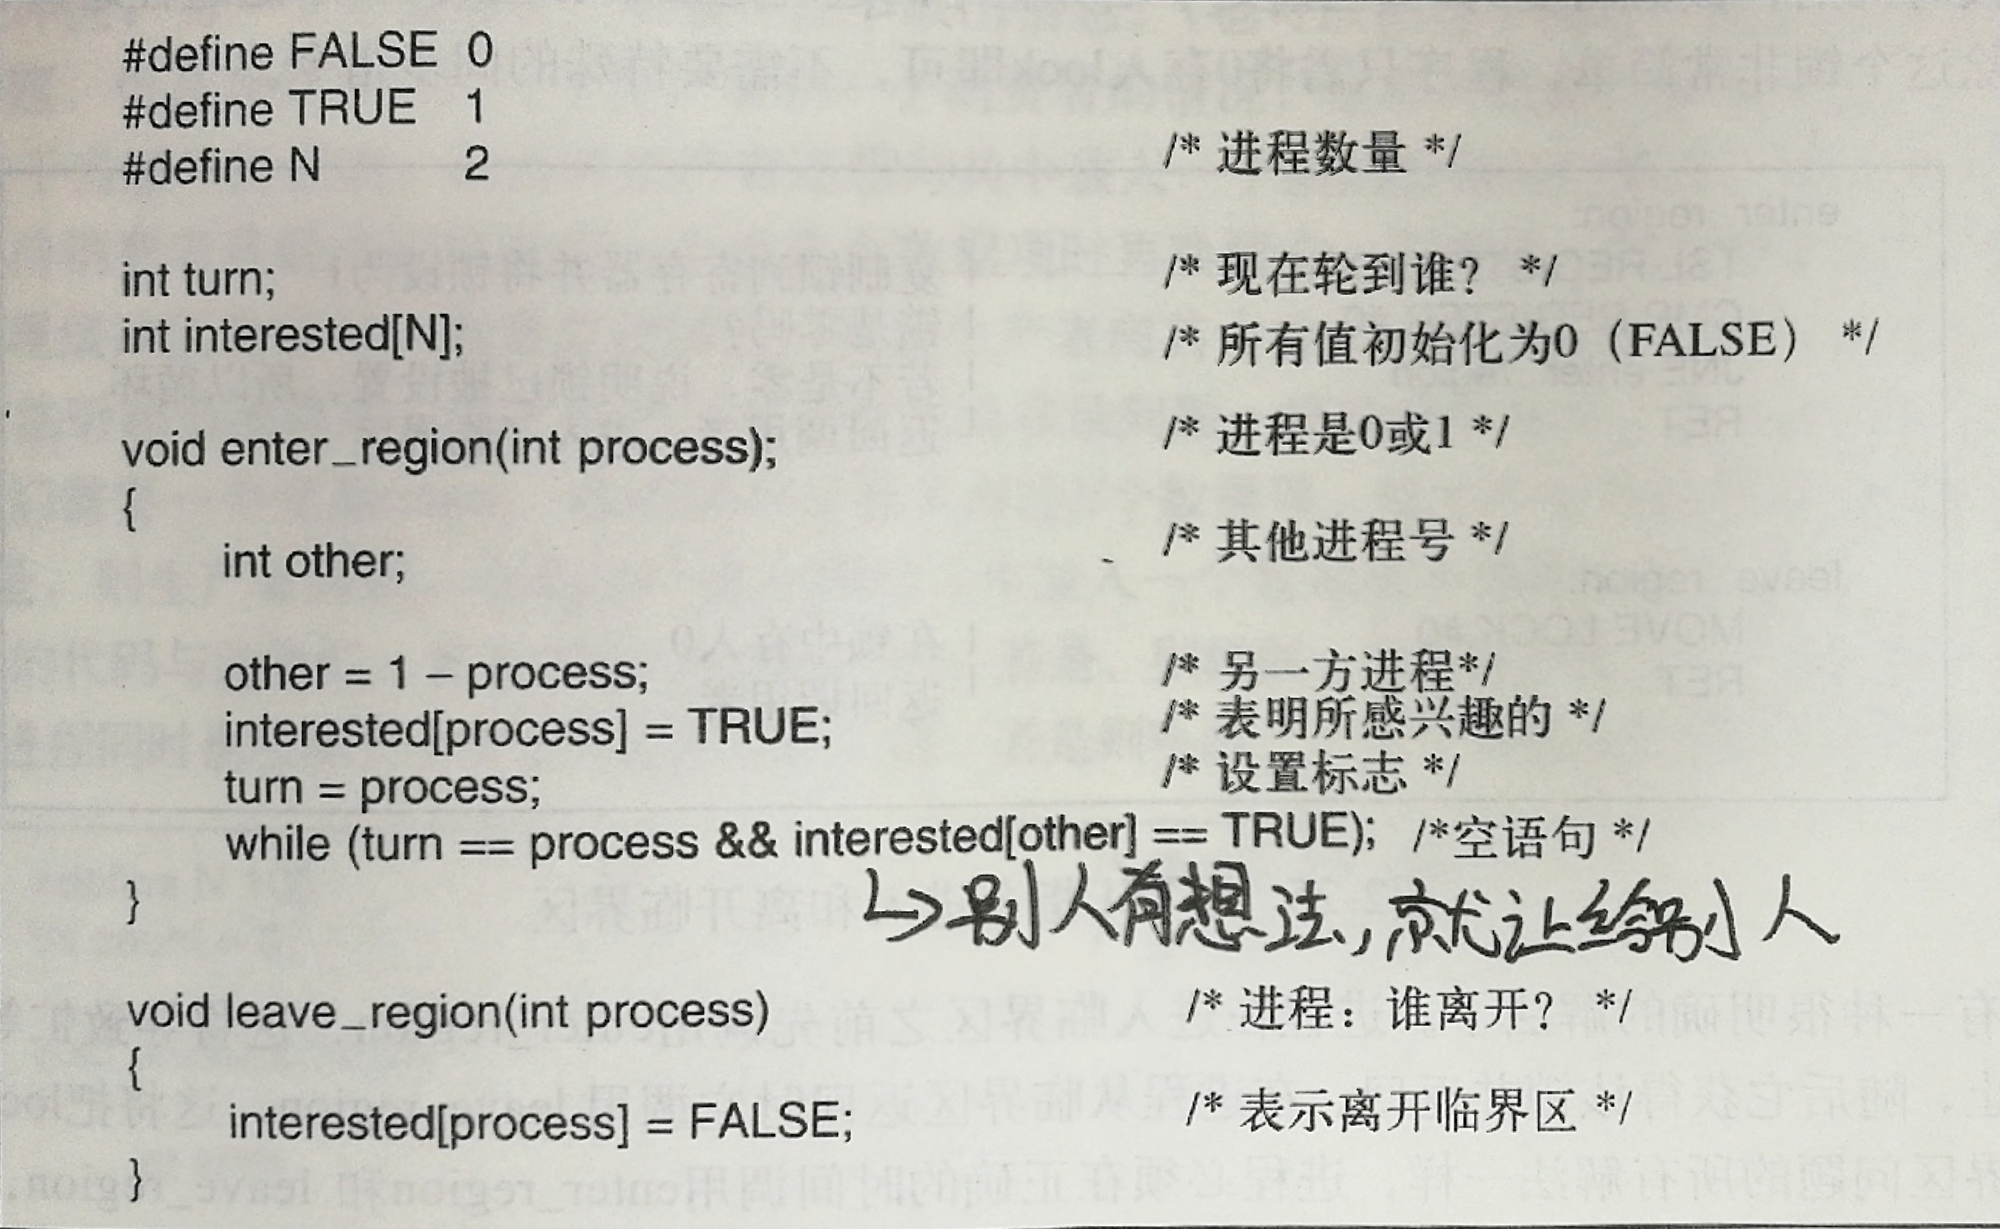
\includegraphics[scale = 0.2]{assets/ModernOperatingSystems_97ad7.png}
        \caption{Peterson解法}
      \end{figure}
      增加了一个所谓的意愿变量,在进入临界区前,先考虑别人的意愿,如果其他人也有需求,则进入循环等待。\\
      考虑两个进程几乎同时调用$enter\_region$的情况,\\
      他们都将自己的进程号存入$trun$,但只有后保存进去的进程号才有效,前一个因被重写而丢失。\\
      假设进程1是后进入的,那么进入到循环的时候,进程1 将循环等待,而进程0则成功进入临界区。\\
      因此,不会出现死锁的情况。

      {\color{blue}似乎只使用于双进程的情况?}
      \item TSL 指令(Test and Set Lock)\\
      锁变量法出问题的原因,是测锁和加锁两步是分开执行而导致的冲突。\\
      TSL则是一次执行这两个操作。\\
      执行TSL指令的CPU将锁住内存总线,以禁止其他CPU在本指令结束之前访存。\\
      一个可替代TSL指令是\textbf{XCHG},它原子性地交换两个位置的内容。
      \end{itemize}
      \subsubsection{睡眠唤醒}

      忙等的缺点是会循环等待进入临界区,这浪费了CPU时间,一个可选的方案是使用 \textbf{睡眠}和\textbf{唤醒}的方法。

      自动睡眠(阻塞):当无法进入临界区的时候程序进入阻塞状态。

      被动唤醒:当一个进程退出临界区的时候,唤醒下一个访问临界区的进程

      这个方法并不是很好,可能会出现一个进程想要睡眠却被另一个进程唤醒的情况。

      \subsubsection{信号量 Semaphore}
      信号量与变量的区别:信号量的操作都是原子性的。

      一旦一个信号量操作开始,则在该操作完成或阻塞之前,其他进程均不得访问该信号量。

      一个信号量有两个部分组成,一个是资源的数量,一个是等待资源的列表。

      信号量主要有两个操作:
      \begin{itemize}
        \item down\\
        申请资源,同时资源数减一(down 1) ,如果减一之后资源数为0 ,则把这个进程加入到等待列表中
        \item up\\
        释放资源,同时资源数加一(up 1) ,如果加一之后资源数还是小于等于0,则从等待资源的进程列表中取出一个进程唤醒
      \end{itemize}

      \subsubsection{互斥量 mutex}
      互斥量是信号量的一个简化版本,它只有两个状态:解锁和加锁。

      有以下几对指令形式,取其中一种表示即可:
      \begin{itemize}
        \item down-up
        \item wait-signal\\
        首先申请(等待)到资源才能继续
        \item lock-unlock\\
        首先先加锁才能继续
      \end{itemize}

      \subsubsection{管程 Monitor}
      在管程内,任意时刻只有一个活跃进程。\\
      具体例子:java 的 synchronized关键字(被这个关键字标记的方法,同一时间只有一个能运行)
      \begin{figure}[H]\centering
        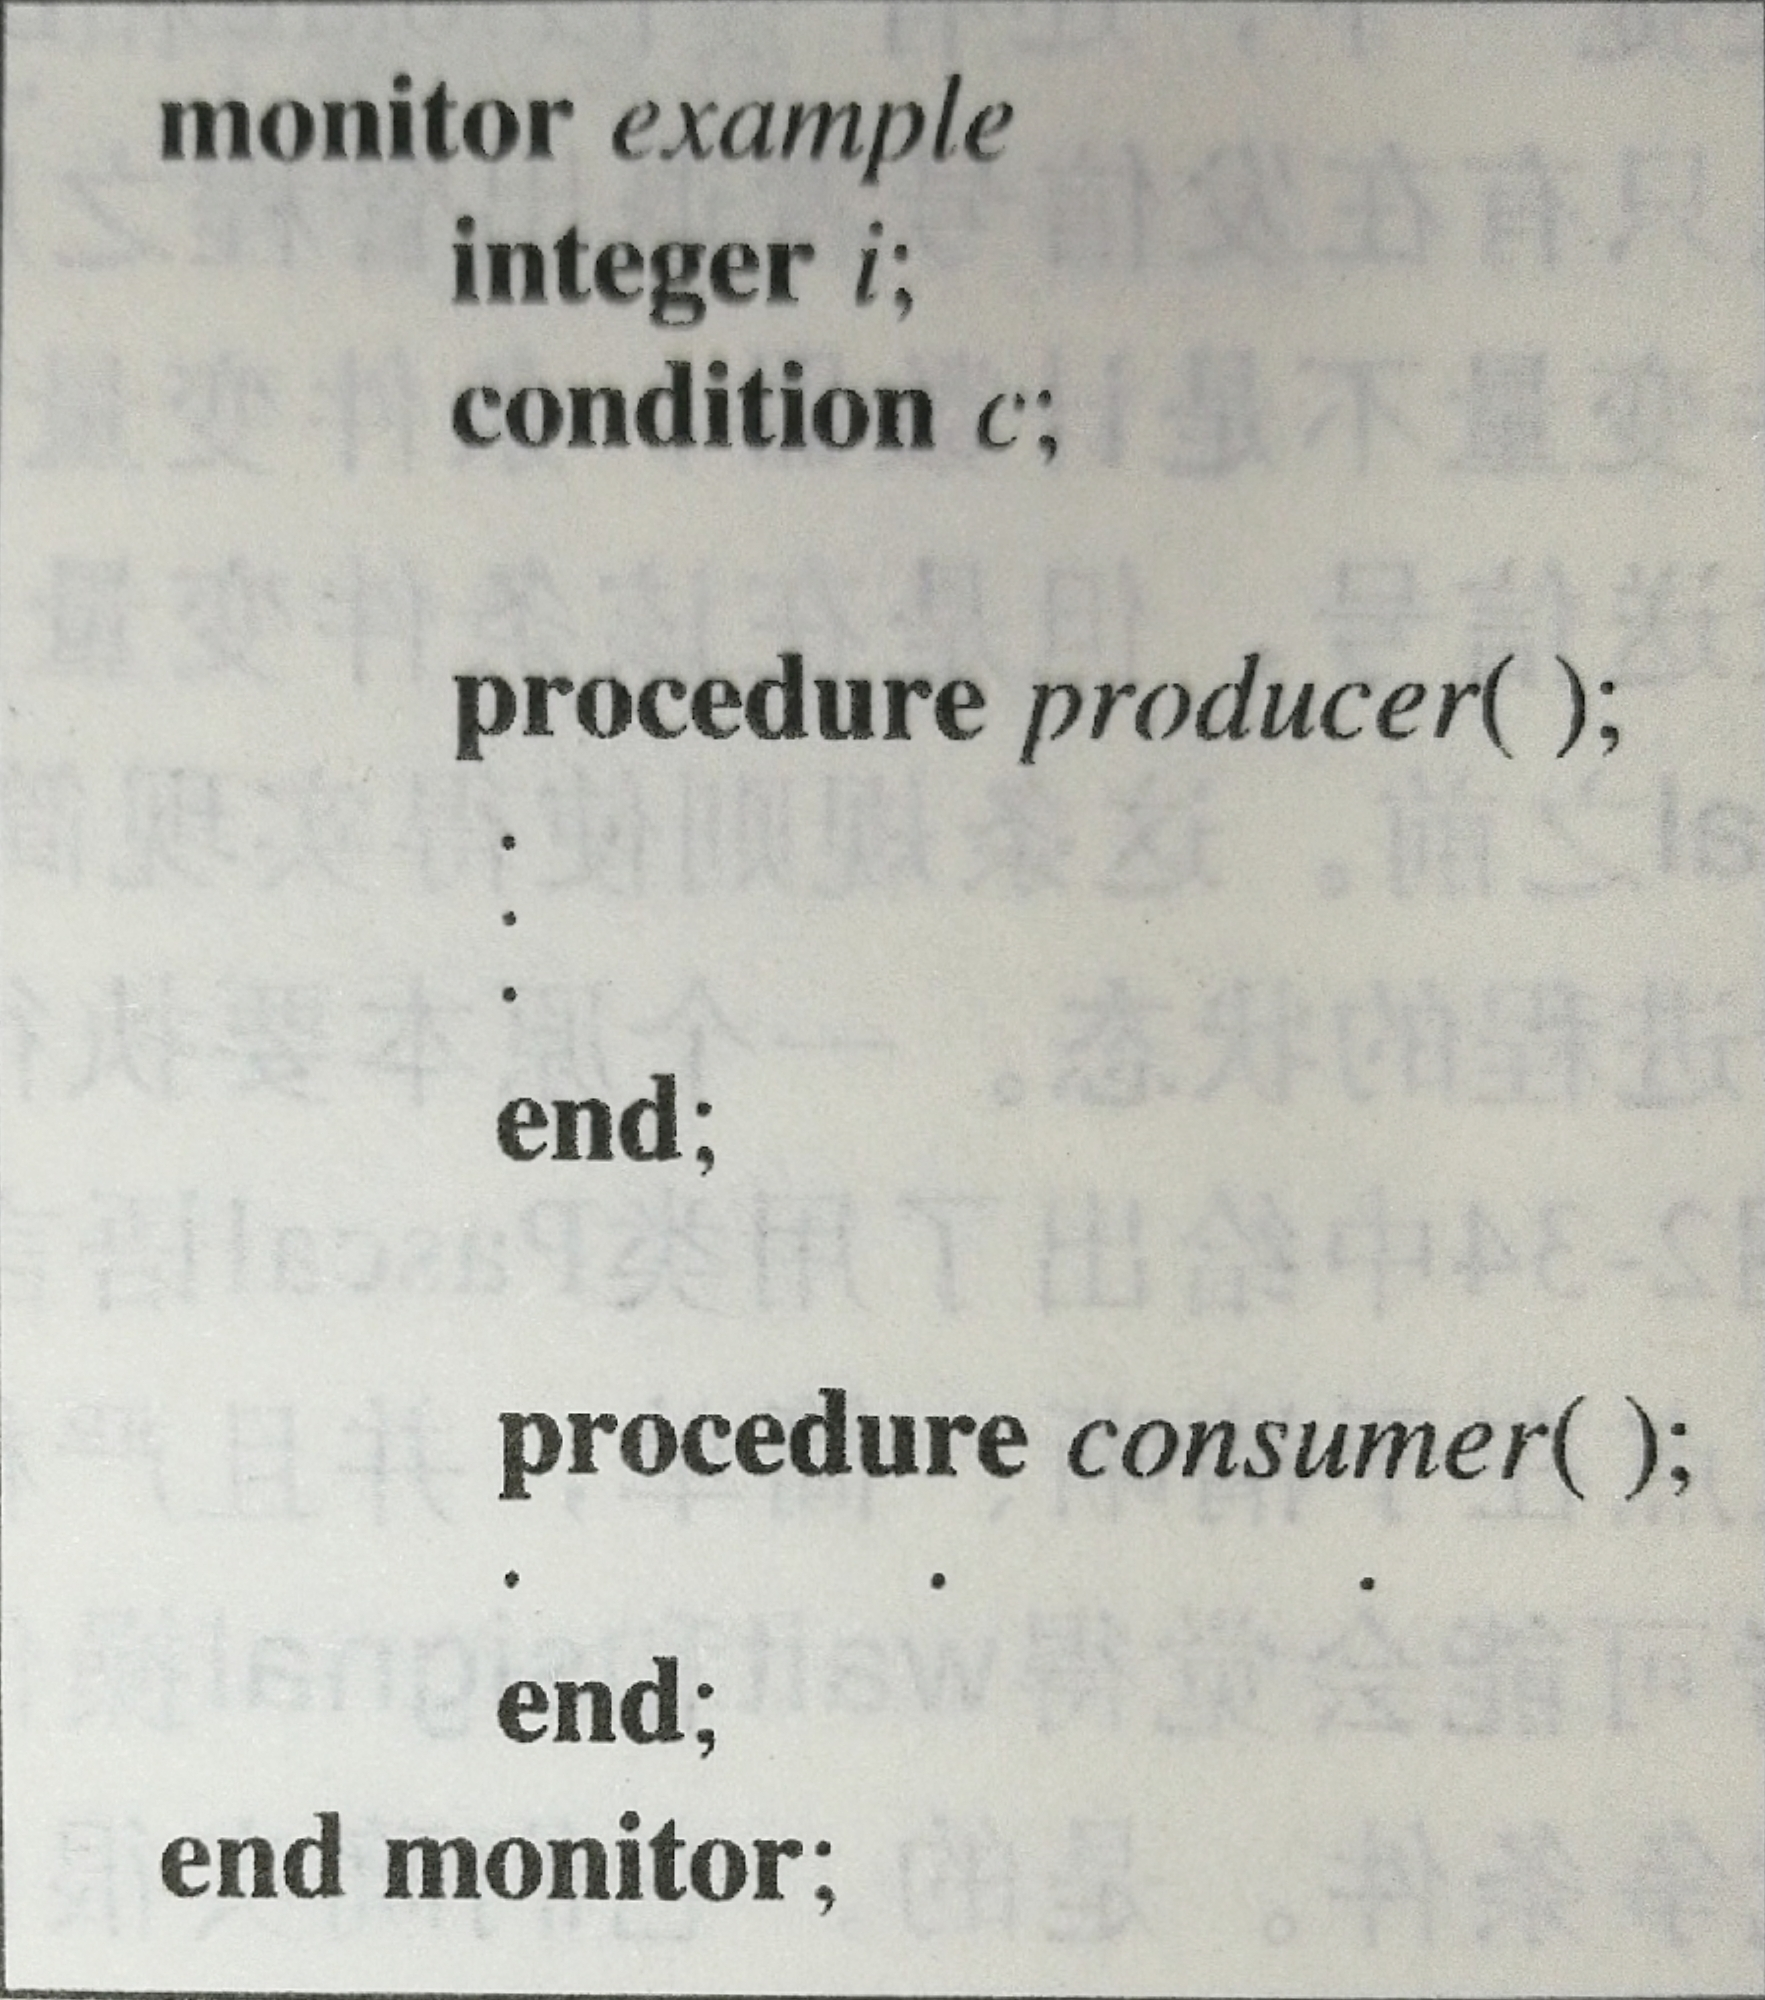
\includegraphics[scale = 0.1]{assets/ModernOperatingSystems_f64a5.png}
        \caption{管程}
      \end{figure}
      \begin{figure}[H]\centering
        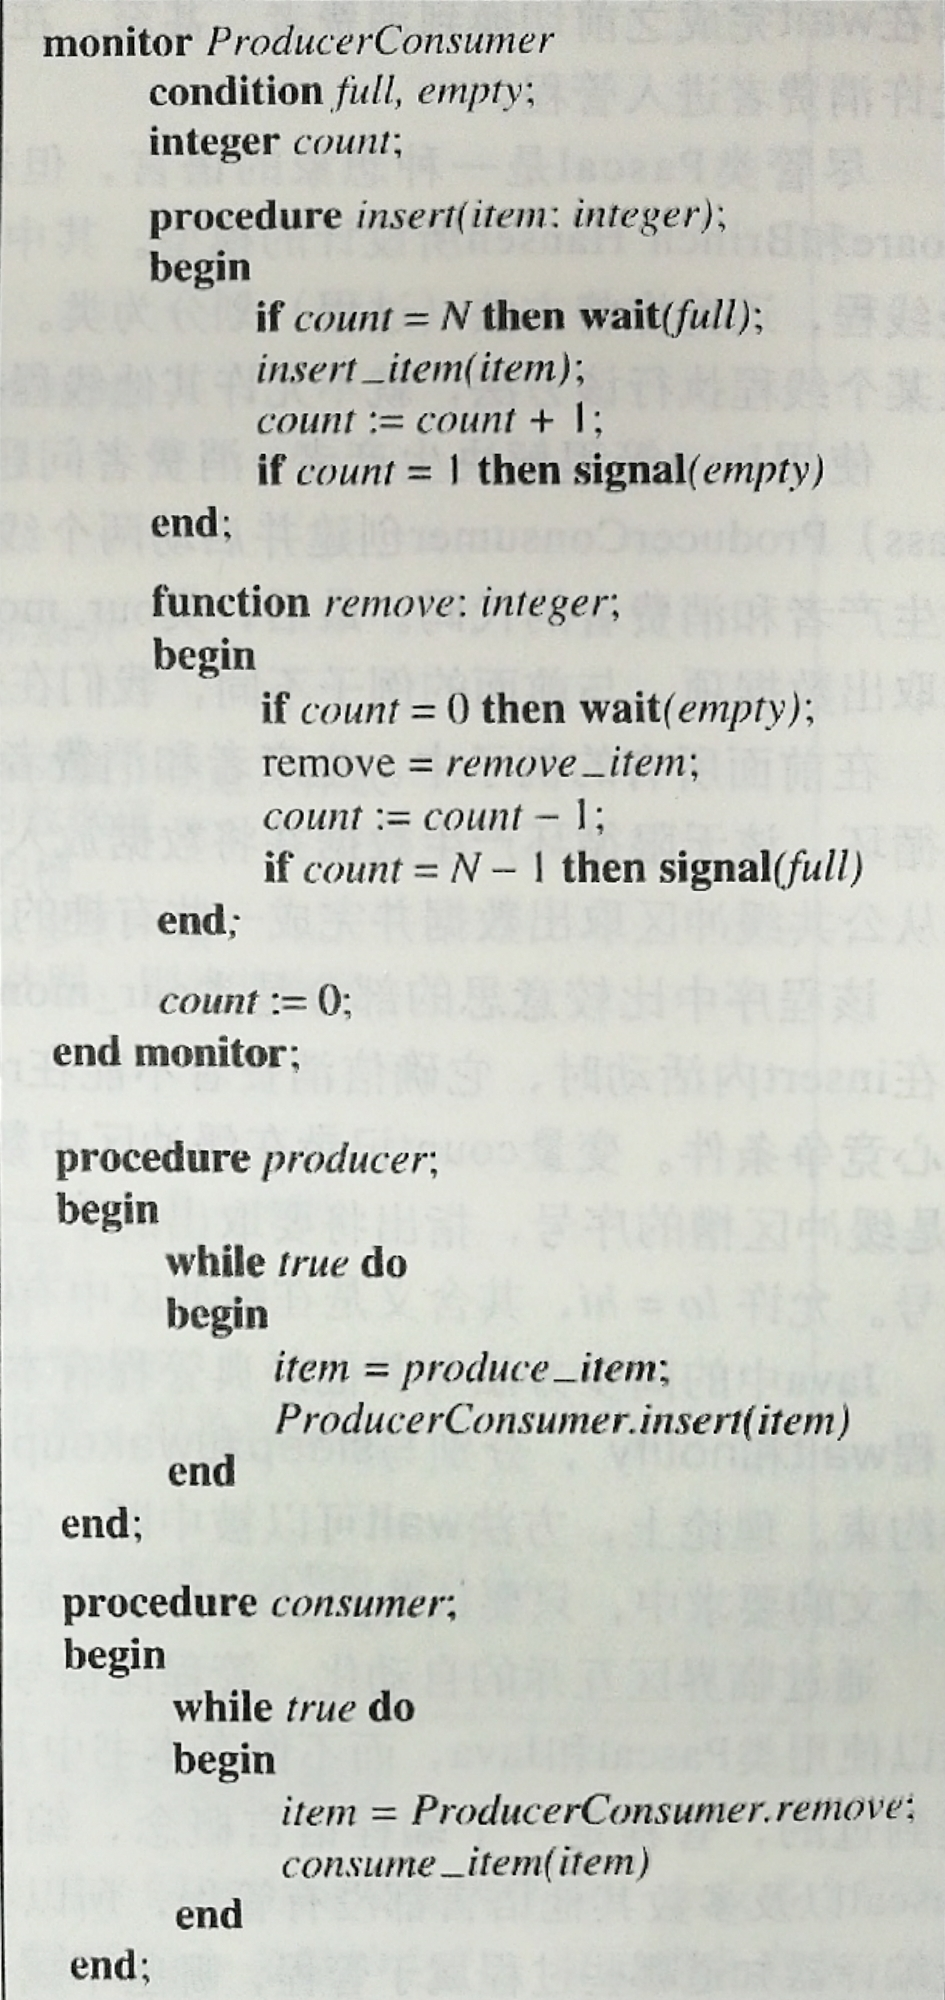
\includegraphics[scale = 0.3]{assets/ModernOperatingSystems_061b9.png}
        \caption{使用管程实现的生产者和消费者问题多的解法框架。}
      \end{figure}

      \subsubsection{消息传递}
      使用消息传递(send/receive)进行通讯,这种进程通讯的方法是使用系统调用而不是语言成分。

      主要有两大类:
      \begin{itemize}
        \item 有缓冲
        \item 无缓冲\\
        在发送之后,进入阻塞直到对方确认
      \end{itemize}

      \subsubsection{屏障}
      屏障:进程组内所有进程就绪之后才进入下一个阶段。

    \subsubsection{5个经典的 ICP问题}

    \paragraph{生产者消费者问题}

    {\color{red}后面补上各种策略}

    \paragraph{环形缓冲区问题}

    {\color{red}没讲}

    \paragraph{读者写者问题}
    多个读者可以同时读取,同时只有一个读者能写,并且不能同时读写。
    问在怎么不死锁的情况下按规则进程读写?

    解决方法:
    \begin{itemize}
      \item 第一次读写的时候加锁,最后读写的时候解锁。
      \item 在控制上面的加锁判断的时候,需要进行互斥操作(即要套上另一个锁再进行加锁解锁的判断和操作)
    \end{itemize}

    \paragraph{哲学家问题}
    哲学家思考和吃面条。

    解决办法:保证操作的原子性,一次必须同时取左右两边两个叉子,不能取则放弃

\end{document}
